%!TEX root = ../Security&NetworkManagement.tex
\chapter{Elementi di crittografia}
La crittografia rappresenta un servizio, cioè un asset. Richiamiamo brevemente alcune proprietà che vorremmo fossero garantite da un sistema sicuro:
\begin{itemize}
	\item \textbf{Disponibilità}: il servizio deve essere sempre disponibile. La disponibilità viene violata nel caso di un attacco \textit{DoS} (Denial of Service). La disponibilità del servizio è la cosa più difficile da garantire, poiché esistono sempre limiti fisici delle risorse e realizzare un attacco DoS deve costare il più possibile. La disponibilità in genere si ottiene con una accurata progettazione della rete.
	\item \textbf{Segretezza}: i dati scambiati devono rimanere riservati tra le parti che partecipano allo scambio. Si tenga presente che le reti ethernet permettono, generalmente, di fare \textit{sniffing} dei pacchetti. Per ottenere questa proprietà si devono utilizzare algoritmi di crittografia (simmetrici, asimmetrici, distribuiti, etc.).
	\item \textbf{Integrità}: i dati devono raggiungere la destinazione senza essere stati modificati. È possibile modificare dati cifrati senza decifrarli ricorrendo a degli attacchi di \textit{bit flipping}. Per ottenere l'integrità dei dati è necessario utilizzare delle funzioni di \textit{hashing}.
	\item \textbf{Autenticazione}: chi riceve un'informazione deve essere sicuro che il mittente sia effettivamente quello dichiarato. I protocolli di internet spesso permettono di effettuare lo \textit{spoofing} degli	indirizzi mittente, ad esempio per le email. È diversa dalla segretezza, perché in questo caso è possibile autenticare anche un messaggio pubblico.
	\item \textbf{Non ripudiabilità}: chi invia un messaggio non può in seguito negare di averlo mandato. Questa proprietà è importante soprattutto a livello applicazione nello scambio di documenti.
	\item \textbf{Anonimato}: rappresenta la possibilità di immettere informazioni in una rete senza che queste siano direttamente collegabili all'identità del mittente. Esistono molte reti anonimizzanti, fra cui Tor, Freenet e remailer anonimi. In genere l'anonimato è richiesto perché si vogliono commettere atti illeciti senza essere rintracciati o perché non si è in condizione di esercitare i propri diritti civili.
\end{itemize}

\section{Principi di crittografia}
Il termine crittografia viene dalle parole greche \textit{kryptós} che significa nascosto, e \textit{gráphein} che significa scrivere. È quindi la scienza che si occupa di rendere segrete le informazioni.

La crittografia ha una storia secolare, dal cifrario di Cesare in poi sono stati fatti molti passi avanti. Oggi nella crittografia confluiscono studi mirati ad ottenere segretezza ma anche tutti gli altri servizi di sicurezza che abbiamo visto; fa eccezione la disponibilità, che ha poco a che vedere con la crittografia, anzi, generalmente un uso troppo diffuso di tecniche di cifratura aumentano la possibilità di essere vittime di DoS.

La crittografia garantisce la \textit{protezione dei documenti} (integrità, segretezza, autenticazione e non ripudiabilità) e la \textit{verifica dell'identità dei corrispondenti} (e.g. tramite il controllo degli accessi).

Per spiegare i principi di base della crittografia useremo degli esempi svincolati da qualsiasi tecnologia, dove vengono coinvolti. Supponiamo che due identità $A$ e $B$ vogliano comunicare attraverso lo scambio di un messaggio $M$. In questo momento assumiamo che non sia specificato alcun protocollo, le considerazioni che faremo si applicano alle connessioni TCP così come alla posta tradizionale. Vedremo in seguito come queste tecniche si applicano alle comunicazioni. Una terza entità $E$ è l'attaccante e proverà ad interferire con i servizi di sicurezza di questo scambio. Si suppone che $E$ possa intercettare i messaggi mentre viaggiano, leggerli e sostituirli così come avviene per un router nella rete Internet.

Le funzioni crittografiche che andremo a vedere sono di più tipi: funzioni hash, funzioni di cifratura a chiave simmetrica e funzioni di cifratura a chiave pubblica/privata. Da queste si derivano funzioni di firma digitale e certificazione degli utenti.

\subsection{Funzioni hash e HMAC}
Le funzioni hash risolvono il problema della garanzia di integrità di un documento o messaggio trasmesso. Una funzione hash è una funzione $h$ unidirezionale non invertibile
\begin{eqnarray*}
h:\mathbb{R}^n\to\mathbb{R}^m & & \text{con } m << n\text{,}\
\end{eqnarray*}
che si applica ad un'informazione (qualsiasi informazione in binario, una email, un pacchetto, un file, etc.) e genera un'impronta di dimensione fissa (un \textit{digest} che può essere di 128, 160, 256... bit) che è funzione dei dati in ingresso. Nel caso di messaggi a dimensione variabile si applica un hash a blocchi e successivamente si applica un altro hash agli hash ottenuti. Generalmente le funzioni hash sono sequenze di operazioni elementari quali shift e XOR sui dati, sono quindi molto veloci da computare. Si noti che le funzioni hash sono diverse dai CRC: quest'ultimi infatti si occupano di rilevare e correggere gli errori introdotti dal canale di trasmissione. In realtà la funzione hash non ha necessità di essere calcolata velocemente (come un CRC), poiché deve essere \textit{robusta}: messaggi diversi devono necessariamente avere hash diversi. Ad esempio, CASO e COSA hanno lo stesso CRC, ma hash diverso.\\
Un esempio di hash è lo SHA (Figura \ref{img:SHA}).
\begin{figure}[htbp]
	\centering
	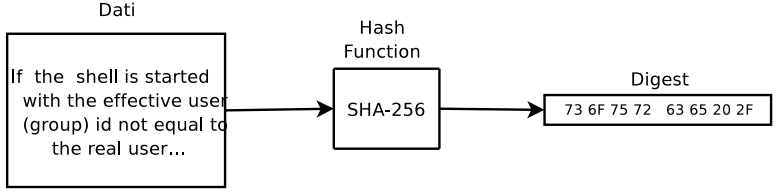
\includegraphics[scale = 0.5]{images/SHA}
	\caption{SHA-256.}
	\label{img:SHA}
\end{figure}
Dato un messaggio $x$, applicando lo SHA otteniamo la \textit{signature} (\textit{digest}) $h(x)$ del nostro messaggio. È molto importante che il messaggio e $h(x)$ siano inviati separatamente, perché se così non fosse si perderebbero le idee e le proprietà fondamentali dell'hash.
\begin{example}[Esempio di utilizzo delle funzioni hash]$\\$
Supponiamo che $A$ invii a $B$ il messaggio $M$ e che invii separatamente anche il digest $d=h(M)$. $B$ riceve quindi $M$ e $d$, e ricalcola $d'=h(M)$: se $d=d'$, allora il messaggio non è stato modificato durante il percorso. La domanda che sorge spontanea è quindi: $E$ cosa può fare? Se $E$ intercetta solo $M$ può provare a cambiarlo, ma quando $B$ riceverà anche $d$, l'hash non sarà più corrispondente e dunque si accorgerà della modifica avvenuta. Per riuscire a modificare il messaggio da $M$ a $M'$, $E$ dovrebbe riuscire ad intercettare anche $d$ per cambiarlo in $h(M')$.\\
Un'applicazione tipica di hash è quella della distribuzione di immagini di file eseguibili: ogni qualvolta viene scaricato un eseguibile è necessario essere sicuri che sia identico al file che il produttore ha generato; anche un solo bit di differenza può provocarne il mancato funzionamento. Con le ISO dei sistemi operativi, infatti, spesso vi viene dato anche il codice MD5 del file, ovvero il digest creato con la funzione hash MD5.
\end{example}

\newpage
Alcuni esempi di fuzioni hash :
\begin{itemize}
\item \textbf{MD5}: digest da 128 bit (il più veloce ma non sicuro)
\item \textbf{SHA-0}: digest da 160 bit (non sicuro)
\item \textbf{SHA-1}: digest da 160 bit (non sicuro a Febbraio 2017)
\item \textbf{SHA-2}: SHA-224, SHA-256, SHA-512 (sicuro)
\item \textbf{SHA-3}: SHA3-256, SHA3-512 (sicuro)
\end{itemize}

\noindent
Vediamo adesso i \textit{requisiti} che deve soddisfare una funzione hash $h$.
\begin{itemize}
	\item \textbf{Compressione}. La funzione $h$ deve mappare un input $x$ avente lunghezza arbitrariamente finita, in un output $h(x)$ di lunghezza $m$ prefissata.
	\item \textbf{Facilità di calcolo}. Data $h$ ed un input $x$, $h(x)$ deve essere semplice da calcolare.
\end{itemize}
Oltre a queste proprietà elementari si aggiungono:
\begin{itemize}
	\item \textbf{Preimage resistance}. Essenzialmente, per tutti gli output pre-specificati $Y=\{y_1,\dots,y_n\}$, deve essere computazionalmente intrattabile trovare un qualsiasi input $x$ tale per cui, applicando $h$, si abbia come risultato $y=h(x)$, dove $y\in Y$. Ossia: l'attaccante conosce l'hash e cerca di risalire al messaggio avente tale hash.
	\item \textbf{2nd-preimage resistance}. Deve essere computazionalmente intrattabile trovare un secondo input che presenta lo stesso output di un input specificato, i.e. dato $x$ deve essere \textquotedblleft impossibile" trovare una 2nd-preimage $x'\neq x$ tale che $h(x') = h(x)$. Ossia: l'attaccante conosce il messaggio e ne cerca un altro con lo stesso hash.
	\item \textbf{Collision resistance}. Deve essere computazionalmente intrattabile trovare due input $x, x'$ che presentino lo stesso output, i.e. tali che $h(x') = h(x)$, ossia trovare due messaggi diversi che abbiano hash uguale.
\end{itemize}
Si noti che comunque una funzione hash è robusta se la sua entropia è massima, cioè ogni bit della signature viene generato in modo equiprobabile. 

In Figura \ref{img:SHA_example} è riportato un esempio di scambio di messaggio attraverso la funzione hash SHA-1. Come è possibile notare, un ipotetico attaccante potrebbe porsi in corrispondenza della linea tratteggiata; potrebbe cioè modificare il testo del messaggio proveniente dall'entità $A$, calcolarne l'hash ed inviare le due informazioni all'entità $B$. In tal modo non è possibile per $B$ capire se il messaggio è stato modificato o meno.
\begin{figure}[htbp]
	\centering
	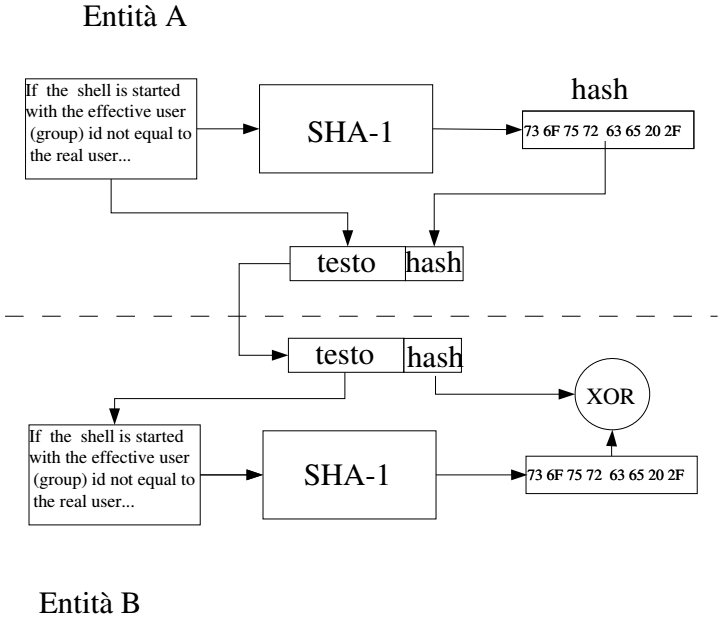
\includegraphics[scale = 0.5]{images/SHA_example}
	\caption{Esempio di trasmissione di un messaggio mediante funzione hash SHA-1.}
	\label{img:SHA_example}
\end{figure}\\
In generale, dunque, le funzioni hash si accompagnano spesso a metodi di \textit{autenticazione}; di seguito ne è riportato uno: HMAC. 

Un HMAC (keyed-\textbf{H}ash \textbf{M}essage \textbf{A}uthentication \textbf{C}ode) accoppia l'utilizzo di una chiave simmetrica ad una funzione hash per garantire, oltre all'integrità, anche l'autenticazione dei dati. Una chiave simmetrica non è altro che una stringa di lunghezza opportuna scelta in modo meno predicibile possibile. Spesso, per generare una chiave simmetrica si usano delle funzioni hash a partire da una password alfanumerica, e.g. $K = \text{md5(password)} = 0\text{x}12ab5893092ba4183f3a345872b34f233$. Se si dispone di una buona funzione hash, si può generare un HMAC componendo la funzione hash con la chiave:
$$HMAC_K(m) = H\left((K' \oplus opad)\; ||\; H\left((K' \oplus ipad)\; || \; m\right) \right),$$
dove $H$ è una funzione hash crittografica, $K$ è la chiave segreta, $m$ è il messaggio che deve essere autenticato, $K'$ è un'altra chiave segreta derivata dalla chiave originale $K$, $||$ denota la concatenazione, $\oplus$ denota l'OR esclusivo (XOR), $opad$ e $ipad$ sono rispettivamente outer e inner padding che rappresentano due sequenze numeriche note (dall'RFC 2104 dell'HMAC) e servono a distinguere i due blocchi di byte che si ottengono. Si nota facilmente a questo punto che il digest può essere calcolato solo se si conosce anche la chiave $K$.
\begin{example}[Uso di un HMAC]$\\$
Supponiamo che $A$ e $B$ si mettano d'accordo su una password. Per mettersi d'accordo devono usare un canale sicuro (si vedono di persona o si telefonano). $A$ per inviare un messaggio $m$ a $B$ compie le seguenti azioni: calcola $K = \text{md5(password)}$, calcola $HMAC_K(m)$ ed invia a $B$ la coppia $\left(m, HMAC_K(m)\right)$. Si noti che le informazioni $\left(m, HMAC_K(m)\right)$ possono essere inviate accoppiate nello stesso pacchetto.
\end{example}
\begin{figure}[htbp]
	\centering
	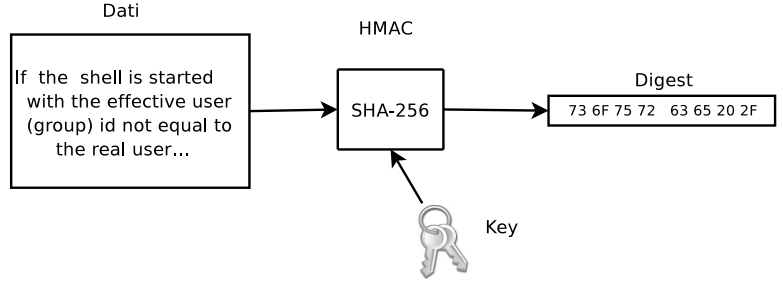
\includegraphics[scale = 0.5]{images/HMAC}
	\caption{Esempio di calcolo di HMAC.}
	\label{img:HMAC}
\end{figure}
Vediamo brevemente i vantaggi rispetto ad una funzione hash. Se $E$ intercetta entrambe le informazioni $m, HMAC_K(m)$ per cambiare il messaggio $m$ dovrebbe modificare $m$ in $m'$ e ricalcolare $HMAC_K(m')$; tuttavia, dal momento che $E$ non è in possesso di $K$ non può calcolare l'HMAC. Schemi di questo tipo vengono utilizzati per garantire l'integrità e implicitamente anche l'autenticazione di pacchetti di livello MAC in molte reti (es. WiFi). Affinché le chiavi siano il più robuste possibile, devono essere generate in modo casuale attraverso un \textit{rumore bianco} per garantire la non correlazione tra i valori generati (motivo per cui si fa l'hash della chiave nell'HMAC).

Vediamo adesso i problemi dell'HMAC. Il primo problema è di gestione: se $A$ e $B$ si devono scambiare una chiave in modo sicuro, un metodo del genere non è utile per comunicazioni via Internet. Il secondo problema sono gli attacchi a forza bruta: $E$ potrebbe intercettare un pacchetto e cercare di indovinare la chiave $K$:
\begin{enumerate}
	\item Dato $m$ e $K=0\text{x}00000000000000000000000000000000$
	\item Il digest $D=HMAC_K(m)$? Se è vero, allora $K$ è la chiave giusta, altrimenti poni $K=0\text{x}00000000000000000000000000000001$ e riprova.
\end{enumerate}
Un attacco di questo tipo è computazionalmente impegnativo: per calcolare tutte le chiavi possibili ($2^{128}$) sono necessari migliaia di anni con i computer di oggi. Tuttavia, se la chiave $K$ è generata da una password, allora l'attacco diventa possibile attraverso ad esempio un dizionario:
\begin{enumerate}
	\item Dato $m$ e $K=\text{md5}(abaco)$, $D=HMAC_K(m)$.
	\item Se è falso, poni $K=\text{md5}(abate)$ e così via.
\end{enumerate}
Le parole di un dizionario potrebbero essere anche alcune decine di migliaia e per generarle tutte ci vogliono pochi minuti. Per questo le password non dovrebbero essere scelte come parole esistenti.

\subsection{Cifratura a chiave simmetrica}
I due elementi principali di un sistema crittografico sono il \textit{cifrario} (un algoritmo) ed una \textit{chiave} (informazione); il metodo si suppone noto a tutti, mentre la chiave deve rimanere segreta. La conoscenza della chiave consente di cifrare/decifrare documenti ed in certi casi può costituire una prova certa di identità. Gli algoritmi di cifratura implementano la segretezza ed a volte l'autenticazione dei dati. Uno dei principi fondamentali è il \textbf{principio di Kerchoffs} che afferma che (1) gli algoritmi crittografici devono essere noti a priori e che (2) un prodotto che garantisce una cifratura con un algoritmo segreto, non è un buon prodotto (se il sistema \textquotedblleft va giù" non sappiamo né come recuperarlo né dove agire per risolvere eventuali problemi).

Vediamo adesso brevemente come funziona una cifratura a chiave simmetrica. Come per un HMAC, due soggetti $A$ e $B$ si accordano su una chiave $K$ od una password da cui generare $K$; solo con la chiave $K$ si possono cifrare e decifrare i messaggi. Generalmente l'algoritmo è lo stesso sia per la cifratura sia per la decifratura. Dunque data una \textit{chiave privata condivisa} $K$ ed un algoritmo (e.g. DES) mittente e destinatario possono codificare e decodificare i messaggi con la chiave scambiata $K$. La robustezza degli algoritmi simmetrici è legata alla lunghezza della chiave: tanto più lungo è il testo della chiave segreta, tanto più difficile è decifrare il messaggio in tempo utile. In genere le chiavi, per essere \textquotedblleft forti", dovrebbero avere una lunghezza di almeno 128 bit.

I problemi di questo tipo di cifratura sono da una parte la necessità di scambiarsi la chiave in anticipo (poca flessibilità di questo strumento), dall'altra si è esposti ad attacchi a forza bruta, anche se più difficili rispetto al caso dell'HMAC. Infatti, per l'attaccante non è facile sapere ad ogni tentativo se il testo decifrato è quello corretto. Per questo motivo le due tecniche possono essere combinate: prima si genera l'HMAC con una chiave $K$, poi si cifra tutto il pacchetto, compreso l'HMAC con una seconda chiave $K'$. In questo modo si è ragionevolmente sicuri di avere segretezza ed integrità dei dati, oltre ad una forma di autenticazione che dipende da come si sono scambiate le chiavi. Questo tipo di approccio si ritrova nelle reti LAN in cui è facile pre-impostare le chiavi segrete a mano sulle macchine. Si noti che la chiave dell'HMAC deve essere diversa da quella simmetrica.

Si noti che la validità della chiave segreta sta nel fatto che, nel caso di due utenti, deve poter esistere una ed una sola chiave segreta. Ma se abbiamo un numero alto di utenti (pensiamo a un servizio bancario via internet) allora dovranno esistere $N$ chiavi segrete, per garantire la comunicazione codificata. Però generare, ad esempio, un milione di chiavi segrete per un milione di utenti comporta, senza dubbio, tempi e spese. Questo problema viene risolto dalla crittografia asimmetrica.

\subsection{Cifratura a chiave asimmetrica}
In questo tipo di crittografia $A$ e $B$ possiedono due chiavi ciascuno: una chiave pubblica $Pub_A$, $Pub_b$ ed una chiave privata $Priv_A$, $Priv_B$. La chiave privata deve essere mantenuta segreta. È fondamentale che $A$ sia l'unico possessore di $PrivA$ (lo stesso vale per $B$). La chiave pubblica invece è pubblica, $A$ può pubblicare la sua chiave $Pub_A$ su Internet rendendola nota a tutti.\\
L'idea (Figura \ref{img:asymmetric_encryption}) è che ciò che viene cifrato con una chiave pubblica può essere decifrato solo con la corrispondente chiave privata; è computazionalmente impossibile risalire ad una chiave privata tramite la chiave pubblica. Se $A$ utilizza la chiave pubblica di $B$ per cifrare un messaggio, allora solo $B$ può decifrarlo, perché è l'unico che possiede la corrispondente chiave privata. Si ottiene quindi il servizio di sicurezza della \textit{segretezza}.
\begin{figure}[htbp]
	\centering
	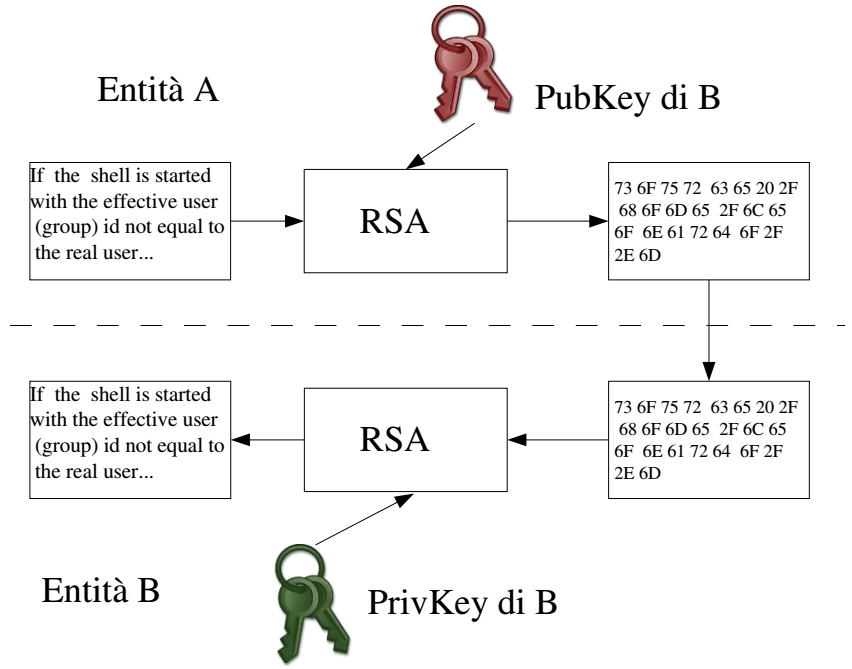
\includegraphics[scale = 0.6]{images/asymmetric_encryption}
	\caption{Esempio di cifratura a chiave asimmetrica.}
	\label{img:asymmetric_encryption}
\end{figure}\\
Ricapitolando, ogni utente ha due chiavi legate in modo inscindibile che possono essere generate insieme da programmi appositi: una chiave viene resa pubblica (possibilmente in un elenco pubblico accessibile da chiunque), mentre l'altra è in possesso del solo utente. Non è necessario concordare preventivamente una chiave di cifratura comune per scambiarsi un documento riservato. La chiave privata di un utente è sempre segreta.

Le chiavi pubblica e privata sono invertibili: se $A$, che è l'unico possessore della chiave $Priv_A$, usa questa chiave privata per cifrare un messaggio, allora chiunque possegga $Pub_A$ può decifrarlo. Siccome $Pub_A$ è pubblica la possiedono tutti, dunque il messaggio è decifrabile da chiunque. Ma, dato che solo $A$ è in possesso di $Priv_A$, chi decifra il messaggio è sicuro che il messaggio provenga direttamente da $A$. Con questo utilizzo la cifratura a chiave asimmetrica non serve a garantire segretezza ma serve a garantire l'autenticazione del mittente. Questo tipo di uso si chiama \textbf{firma digitale} (Figura \ref{img:digital_signature}) e fornisce l'autenticazione e non la ripudiabilità dei dati. Posso quindi mandare messaggi in chiaro e accodare l'hash cifrato del messaggio. Questo perchè posso verificare sempre che l'HMAC è effettivamente mandato da A (autenticazione, come già detto in precedenza).
\begin{figure}[htbp]
	\centering
	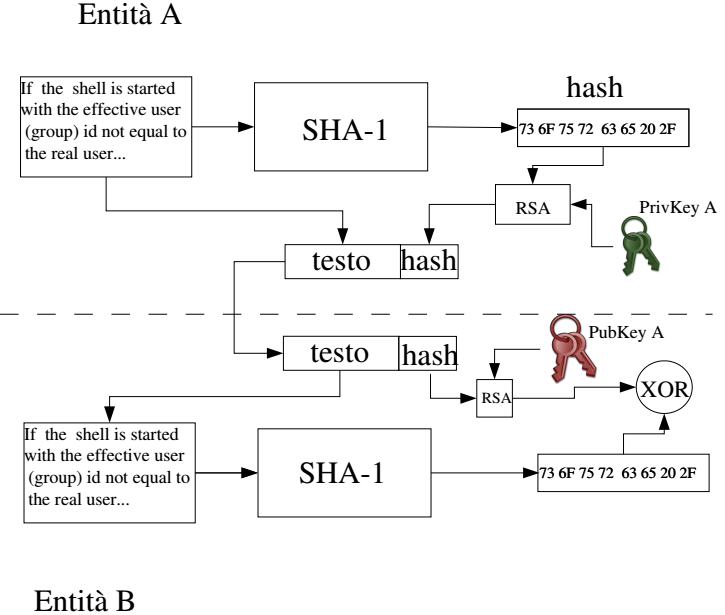
\includegraphics[scale = 0.5]{images/digital_signature}
	\caption{Esempio di firma digitale.}
	\label{img:digital_signature}
\end{figure}\\
Il tipico attacco che si può compiere contro una cifratura asimmetrica è il man-in-the-middle (MITM) che è possibile quando $A$ e $B$ non possiedono le chiavi l'uno dell'altro. Un esempio classico è il seguente. Supponiamo che $A$ invii a $B$ la sua chiave pubblica $Pub_A$; se $E$ intercetta il messaggio può scambiare la chiave $Pub_A$ con $Pub_E$ e dunque $B$ riceve la chiave $Pub_E$ convinto che sia la chiave di $A$. $B$ invia dunque un messaggio $M$ cifrato con chiave $Pub_E$, $E$ lo intercetta, lo decifra, lo cifra nuovamente con la chiave $Pub_A$ e lo invia ad $A$. L'entità $A$ riceve quindi il messaggio e lo decifra, ma $E$ ha potuto intercettare il contenuto ed eventualmente modificarlo.

Un attacco MITM è sempre possibile quando $A$ e $B$ non conoscono in anticipo le rispettive chiavi. Le chiavi quindi non devono essere scambiate durante la comunicazione stessa, ma attraverso qualche altro mezzo. Si ricrea dunque il problema visto precedentemente con la chiave simmetrica, ovvero che deve esistere un mezzo \textit{sicuro} attraverso il quale $A$ e $B$ si scambiano la chiave. La grande differenza rispetto al caso precedente è che per \textit{sicuro} non si intende segreto, ma semplicemente autenticato.\\
Per risolvere questo tipo di problema si utilizzano \textbf{fingerprint}, \textbf{keyserver} e \textbf{Web Of Trust}.

Una \textit{fingerprint} è semplicemente una piccola parte dell'hash della chiave pubblica, in particolare i primi 24 byte. È altamente improbabile che due chiavi pubbliche diverse abbiano i primi 24 byte in comune. Il destinatario può facilmente controllare se i messaggi che sta ricevendo provengono dallo stesso mittente verificando che tutti presentino lo stesso fingerprint. Inoltre è molto più semplice distribuire una fingerprint rispetto ad una chiave pubblica; ad esempio, può essere utilizzata come signature nella posta elettronica oppure potrebbe essere inserita in un biglietto da visita. Se riceviamo posta elettronica da qualcuno da anni ed esso usa la sua fingerprint nella signature, il giorno in cui si ha bisogno di utilizzare la sua chiave pubblica lui la invierà e sarà possibile verificare se la chiave ricevuta corrisponde alla fingerprint che lui ha usato in passato.

I \textit{keyserver} sono server pubblici sui quali è possibile caricare le chiavi pubbliche. Il keyserver non garantisce niente: non si fa carico di stabilire l'associazione tra utente e chiave, accetta semplicemente l'upload e il download delle chiavi stesse. Nella chiave si possono inserire informazioni come il nome utente o il suo indirizzo di posta elettronica, quindi cercando in un motore di ricerca è possibile trovare la chiave pubblica di chi vogliamo. Si noti però che trovare la chiave di una certa persona $x$ su un keyserver non dà alcuna certezza sul fatto che $x$ usi veramente quella chiave. I keyserver sono solo un \textquotedblleft modo comodo" per archiviare ed accedere a chiavi pubbliche: è necessario accertarsi che la chiave presa in considerazione corrisponda veramente all'identità dichiarata.
\begin{figure}[htbp]
	\centering
	\begin{tikzpicture}[->,>=stealth',shorten >=1pt,auto,node distance=5cm,
	semithick, scale = 0.6, transform shape]
	
	\node[state] (1) {$KS$};
	\node[state] (2) [left of=1] {$A$};
	\node[state] (3) [right of=1] {$B$};
	\node[state] (4) [below of=1] {$E$};
	
	\path 	(2) edge node {(1) $Pub_A$} (1)
	(4) edge node {(2) $Pub_A$} (1)
	(3) edge node {(3) $Pub_A$?} (1)
	(1) edge [bend left] node {(4) $Pub_A$!} (3);
	\end{tikzpicture}
	\caption{Esempio di \textquotedblleft attacco" ad un keyserver.}
	\label{graph:KS_attack}
\end{figure}\\
In Figura \ref{graph:KS_attack} è riportato un esempio di cambio di una chiave pubblica da parte di un attaccante. La comunicazione fra $B$ ed il keyserver è protetta, dunque $E$ non può stare tra il keyserver e $B$. $E$ può stare tra $A$ ed il keyserver: se $A$ non controlla frequentemente la propria chiave sul keyserver questa potrebbe essere sostituita da quella di un attaccante che quindi sarebbe associato all'identità di $A$.

L'idea di un \textit{Web Of Trust} (\textit{WOT}) è invece quella di creare una rete di contatti attraverso la quale i partecipanti certificano l'identità altrui. Il principio alla base di un WOT è che se $A$ conosce personalmente $B$, allora $A$ può certificare $Pub_B$, ovvero garantire agli altri che una certa chiave pubblica è effettivamente quella di $B$. Se un'entità $C$, pur non conoscendo $B$, conosce $A$, si dice che $C$ ha un livello \textquotedblleft di affidabilità" maggiore nella chiave $Pub_B$ rispetto alla certificazione di un qualche altro utente che non conosce né $A$ né $B$.\\
Ogni utente quindi ha interesse affinché la propria chiave sia certificata dal maggior numero di persone possibile, poiché in tal caso aumenterebbe il proprio livello di \textit{trust}. Le certificazioni avvengono utilizzando la propria chiave privata per firmare la chiave pubblica altrui.
\begin{example}[WOT]$\\$
Supponiamo che $A$ generi la propria coppia di chiavi $Pub_A$ e $Priv_A$. La chiave pubblica contiene l'informazione che tale chiave appartiene ad $A$. A questo punto, $A$ si reca da $B$, gli mostra un documento e gli consegna la fingerprint della chiave; $B$ scarica la chiave da un keyserver e controlla che la fingerprint corrisponda. Da questo punto in poi $B$ può firmare con la propria chiave privata $Priv_B$ la chiave pubblica di $A$, $Pub_A$, e può caricare la chiave firmata sul keyserver.
\end{example}
Il limite di questa tecnica sta nel fatto che un possibile attaccante potrebbe farsi firmare la propria chiave pubblica da tante altre entità che conosce, facendo così crescere il proprio livello di trust ed allo stesso tempo fingersi un'altra entità.

Il primo programma che permetteva agli utenti di generare chiavi pubbliche/private e inviarsi messaggi cifrati è stato PGP (Pretty Good Privacy). Questo programma ha avuto molti problemi di distribuzione all'inizio della sua vita, perché le leggi statunitensi trattavano la crittografia alla stregua di armi e ne vietavano l'\textit{esportazione}. Il PGP in principio era distribuito con il codice sorgente; in seguito il codice sorgente è stato chiuso ed il programma è diventato commerciale. Nacque dunque GPG (GNU Privacy Guard), che implementa le stesse funzioni ma venne rilasciato con una licenza libera, la GNU GPL. GPG può essere usato anche con programmi di posta elettronica come Thunderbird.

Vediamo di seguito alcuni comandi bash utili per utilizzare GPG.\\
I seguenti comandi servono rispettivamente per creare chiavi, esportare chiavi, caricare una chiave su un keyserver e cifrare i messaggi:
\shellcmd{gpg --gen-key}
\shellcmd{gpg --export --armor C93F299D}
\shellcmd{gpg --keyserver pgp.mit.edu --send-key C93F299D}
\shellcmd{gpg --encrypt -r C93F299D file}

\subsection{Certificati}
Il WOT di GPG è comodo, ma si basa sulla fiducia reciproca e sul grande numero di persone che vi partecipano. In contesti più formali, affinché una chiave pubblica sia associata ad una
persona, sono necessarie garanzie più forti che possono essere date solo da terze parti riconosciute: gli \textit{enti certificatori}.\\
Una CA (Certification Authority) è un ente che garantisce l'associazione tra chiave pubblica e persona fisica. L'ente possiede una sua coppia di chiavi pubblica/privata, gli utenti conoscono l'ente (e la sua chiave pubblica) e si fidano delle certificazioni che rilascia. La certificazione avviene esattamente come per le chiavi GPG, ma utilizza un formato di file diverso: lo standard \textsf{X.509}. Alcuni esempi di enti di certificazione sono Poste Italiane e Verisign.

Vediamo adesso più nel dettaglio come avviene la certificazione. L'utente $A$ genera una coppia di chiavi pubblica/privata ed invia all'ente certificatore la propria chiave pubblica ed un documento. L'ente restituisce la chiave pubblica dell'utente $A$ firmata con la propria chiave privata; il contenitore in cui si sposta la chiave è un \textit{certificato}. Si noti che questa procedura è necessaria una sola volta, alla creazione della chiave. In questo modo l'ente certificatore non conosce la chiave privata, che rappresenta quindi una maggiore garanzia dell'utente. In un caso più semplice la CA invia entrambe le chiavi e il certificato all'utente.\\
Quando un secondo utente $B$ deve parlare con $A$, $B$ chiede ad $A$ il suo certificato dal quale estrae la chiave pubblica di $A$ e verifica che la firma digitale dell'ente certificatore sia corretta utilizzando la chiave pubblica dell'ente. A quel punto è sicuro che l'utente $A$ sia veramente chi dichiara di essere, poiché l'ente certificatore è testimone per lui.\\
Nel caso in cui un utente voglia utilizzare la propria firma digitale per qualche scopo, questa risulta valida solo se certificata da un'ente: la firma digitale certificata ha lo stesso identico valore legale della firma manoscritta su carta. Attraverso un sistema di certificati si può ottenere inoltre un accurato controllo degli accessi.
\begin{figure}[htbp]
	\centering
	\begin{tabular}{|c|}
		\hline
		ID ente certificatore \\
		\hline
		Serial Number \\
		\hline
		Periodo di validità \\
		\hline
		Dati del soggetto \\
		\hline
		Chiave pubblica \\
		\hline
		Firma digitale del CA \\ \hline
	\end{tabular}
	\caption{Campi principali di un certificato.}
	\label{tab:certificate}
\end{figure}\\
In Figura \ref{tab:certificate} sono riportate le informazioni principali presenti in un certificato. Contiene: i dati identificativi dell'entità che svolge il ruolo di garante, un serial number che identifica univocamente il certificato, il periodo di validità, i dati identificativi del soggetto (utente o dispositivo) per cui è rilasciato, la chiave pubblica del soggetto e la firma digitale dell'ente che ha emesso il certificato.

Lo stesso modello può essere riprodotto per qualsiasi contesto, anche senza bisogno di contattare una CA ufficiale. Supponiamo, ad esempio, di amministrare la rete in una certa azienda e di avere a disposizione i seguenti servizi: posta elettronica per gli utenti, sito web e rete interna a cui collegare computer fissi e portatili. È possibile creare una propria CA avente una coppia di chiavi ed il certificato. In questo caso il certificato è \textit{autofirmato}, ovvero la CA certifica sé stessa. Con questa CA è possibile quindi rilasciare certificati validi per tutti gli utenti, in modo che possano inviare solo posta elettronica firmata digitalmente. Ogni volta che un utente riceve una e-mail questa è autenticata e cifrata. I browser installati sui computer aziendali possiederanno un certificato proprio: in tal modo il server può accettare connessioni solo dalle macchine utilizzate. Quando un portatile si connette alla rete, prima di essere abilitato a trasmettere e ricevere traffico, dovrà autenticarsi con un server utilizzando un certificato valido. Generalmente, piuttosto che non avere un certificato, è meglio averlo autofirmato, perché si presume che la chiave privata del CA ipotetico sia diverso da un altro CA con lo stesso nome usato dell'attaccante.\\
Dunque anche se la CA non è ufficiale è possibile utilizzarla all'interno della propria organizzazione per aumentare il livello di sicurezza delle comunicazioni. È inutile sottolineare che se per qualche motivo il server su cui risiedono le chiavi pubbliche e private della CA viene compromesso, automaticamente è compromessa anche la sicurezza di tutta la rete.\\
Ipotizziamo, adesso, di avere davanti uno dei seguenti scenari:
\begin{itemize}
	\item Un utente perde il portatile con dentro un certificato valido;
	\item Uno dei server con un certificato viene compromesso;
	\item Si scopre che un utente si \textit{comporta male}.
\end{itemize}
In questi casi la cosa da fare è quella di revocare le credenziali di alcuni utenti, ovvero riuscire ad invalidare i certificati già rilasciati. Per farlo ricorriamo alle \textit{Certificate Revocation List} (CRL). Una CRL è semplicemente una lista di certificati che sono stati revocati dall'ente certificatore. Revocare un certificato significa che il certificato non deve essere più utilizzato; nella pratica avviene che la CA mantiene una lista di certificati non più validi e la distribuisce firmandola con la sua chiave privata. Nella gestione di una rete sicura quindi si deve tenere conto anche del fatto che deve esistere un servizio attraverso il quale un utente può scaricare la CRL più aggiornata. Le CRL introducono un elemento di complicazione in più ma sono necessarie: rendono infatti i certificati non più autonomi (auto-verificabili), ma emerge la necessità di richiedere un parere ad un ente terzo.

Vediamo adesso un \textit{approccio misto}: il WOT di Thawte. Thawte è un'azienda che possiede una CA autorizzata, ma rilascia anche certificati secondo la logica del WOT. Thawte ha dei \textit{notai}. I notai possono certificare altre persone, pur non essendo direttamente dipendenti di Thawte. Nella pratica funziona nel seguente modo: si crea un account Thawte e si va da un notaio portando il numero dell'account creato ed una fotocopia di due documenti. Il notaio ha il potere di accedere al sito di Thawte ed accreditare dei \textit{punti} sull'account personale creato. Non appena si raggiunge un numero sufficiente di punti, viene da Thawte consegnato un certificato per la propria identità \textit{rilasciato dalla CA autorizzata di Thawte}. Continuando ad incontrare notai è possibile accumulare punti fino a diventare noi stessi notai. Chiaramente i domini dei certifcati Thawte per il WOT e per le attività commerciali sono separati. Questo modello tuttavia non ha avuto molto successo, poiché dal punto di vista del business non è molto buono.

Un esempio di programma per gestire una certification authority è TinyCA. Attraverso questo programma è possibile generare certificati e firmare chiavi pubbliche.

\subsection*{Riepilogo}
Finora abbiamo visto sostanzialmente due tipi di crittografia: simmetrica e asimmetrica. La crittografia simmetrica ha bisogno di un canale sicuro per lavorare, cosa che non è necessaria in quella asimmetrica. L'aspetto positivo della crittografia simmetrica è che è \textit{computazionalmente semplice} in quanto la complessità computazionale è dipendente dalla lunghezza della chiave (corta). Questo aspetto non è vero nella crittografia asimmetrica: si ha a che fare con chiavi lunghe che rendono gli algoritmi computazionalmente molto pesanti. Si noti che la complessità computazionale è direttamente proporzionale alla sicurezza della chiave. Solitamente le due tecniche vengono utilizzate insieme per garantire sicurezza e performance.

Vediamo quindi un esempio di un possibile sistema misto per la sicurezza dello scambio di informazioni tra $A$ e $B$\footnote{con $\{x\}_y$ si indica il messaggio $x$ cifrato con la chiave $y$.}:
\begin{enumerate}
	\item $A\to B$: $A$ manda a $B$ il proprio certificato $C_A$.
	\item $A \leftarrow B$:  $B$ manda a $A$ il proprio certificato $C_B$.
	\item $A\to B$: $A$ genera un numero casuale $R$ e trasmette $\{R\}_{C_B}$.
	\item $A\leftarrow B$: $B$ genera un numero casuale $P$ e trasmette $\{P\}_{C_A}$.
\end{enumerate}
La chiave segreta generata è $K=hash(P\oplus R)$ ($\oplus$ è l'operazione di XOR). Dopo lo scambio effettuato le due parti possono smettere di utilizzare le chiavi pubbliche e continuare a cifrare ed autenticare il traffico solo con la chiave $K$, in modo computazionalmente vantaggioso. Si noti che il precedente algoritmo è una semplificazione di quelli reali e presenta molti difetti: in pratica serve solo a rendere l'idea del funzionamento di algoritmi più complessi come l'RSA.

\section{Cenni teorici}
\begin{defn}[Campo]$\\$
	Un campo finito $\mathbb{F}$ è un insieme di elementi con due operatori ($+$ e $\cdot$) tali per cui valgono le seguenti proprietà: chiusura rispetto alla somma, associatività della somma, identità additiva, inverso additivo, commutatività della somma, chiusura rispetto al prodotto, associatività del prodotto, leggi distributive, commutatività del prodotto, identità moltiplicativa, annullamento del prodotto ed inverso moltiplicativo.
\end{defn}
\begin{defn}[Campo $\mathbb{Z}_n$]$\\$
	Il campo $\mathbb{Z}_n$ è il campo ottenuto dall'insieme dei numeri interi in $[0,n-1]$, dove $n$ è un numero primo, considerando le operazioni di $+$ e $\cdot$ modulo $n$.
\end{defn}
\noindent
Se $a, n$ sono interi, si definisce $a\bmod n$ come il resto della divisione di $a$ per $n$. Le operazioni in modulo sono la somma
$$[a\bmod n + b\bmod n]\bmod n = (a+b)\bmod n$$
e la moltiplicazione
$$[a\bmod n \cdot  b\bmod n]\bmod n = (a\cdot b)\bmod n$$
Inoltre, per qualsiasi elemento $a\in\mathbb{Z}_n$ esiste un unico $a^{-1}$ tale per cui $a\cdot a^{-1} = 1\bmod n$, ovvero un unico inverso moltiplicativo.
\begin{defn}[Funzione Toziente di Eulero $\phi(x)$]$\\$
	La funzione Toziente di Eulero $\phi(x)$ è il numero di interi positivi minori di $x$ e primi relativi di $x$. Si dimostra che se $p, q$ sono due numeri primi e $x=p\cdot q$, allora $\phi(x)=(p-1)(q-1)$.
\end{defn}
Si noti che calcolare $\phi(x)$ per un qualsiasi $x$ è computazionalmente oneroso, impossibile per $x$ sufficientemente grandi. Se $x=p\cdot q$ e conosciamo $x$ ed almeno uno tra $p$ e $q$ è invece possibile calcolare l'altro.
\begin{thm}[di Eulero]$\\$
	Siano $a, x$ primi tra loro. Allora $a^{\phi(x)}=1(\bmod x)$.
\end{thm}
\noindent
Gli algoritmi di crittografia in generale si basano su due principi:
\begin{enumerate}
	\item Il messaggio cifrato deve essere sicuro e non deve essere possibile tornare al messaggio originale da parte di terzi;
	\item Dato un messaggio cifrato, anche avendo un possibile messaggio originale, non deve essere possibile risalire alla chiave originaria. Questo meccanismo è realizzato attraverso una \textit{funzione trappola} (fattorizzazione di un numero primo). Un esempio è il Teorema di Eulero.
\end{enumerate}
Nel seguito vedremo alcuni degli algoritmi crittografici più famosi ed utilizzati.

\subsection{RSA}
RSA è un algoritmo di crittografia asimmetrica inventato nel 1977 da Ronald \textbf{R}ivest, Adi \textbf{S}hamir e Leonard \textbf{A}dleman utilizzabile per cifrare o firmare informazioni. Vediamone brevemente l'idea.

Dati $p, q$, primi tra loro e abbastanza grandi, e $n=p\cdot q$, dato $m$ un numero di dimensione inferiore a $n$ ($m$ può essere la codifica binaria di qualsiasi testo in chiaro), si dimostra che se $e, d$ sono inversi moltiplicativi modulo $\phi(n)$, ossia $ed=1\bmod\phi(n)$, allora
\begin{align*}
	m^{ed}&\bmod n && \\
	=m^{1+k\phi(n)}&\bmod n && \\
	=m(m^{k\phi(n)})&\bmod n && \\
	=(m\bmod n)(m^{k\phi(n)})&\bmod n && \\
	=(m\bmod n)((m^{\phi(n)})^k)&\bmod n && \\
	=m&\bmod n && \text{(per il Teorema di Eulero)}
\end{align*}
Dato $c=(m^e) (\bmod\;n)$ è computazionalmente oneroso ricavare $m$, impossibile per numeri grandi. Quindi è possibile cifrare un messaggio $m$ semplicemente calcolando $(m^e)(\bmod\; n)$ ed è possibile decifrare il messaggio criptato elevandolo alla $d$ e calcolandone il modulo. Dunque la coppia $(e, n)$ costituisce la chiave pubblica, mentre la coppia ($d, n$) la chiave privata. Ad oggi, per valori di $(e, n)$ non piccoli ($> 1$ Kbit), non esistono algoritmi che permettono di ricavare $d$, data la coppia $(e, n)$, e $m$, dato $c$.

Vediamo adesso i possibili attacchi all'RSA. La sicurezza di RSA si basa sull'impossibilità di derivare $\phi(x)$ o $d$ a partire da ($e, n$). Entrambi questi problemi hanno complessità equivalente a quella di \textit{fattorizzare} $n$ nei suoi fattori primi. Tra il 1991 ed il 2003 sono stati fattorizzati numeri da 332 a 663 bit utilizzando algoritmi di fattorizzazione diversi in decine di macchine in cluster a lavoro per mesi. Ad oggi si ritiene che utilizzare chiavi di dimensione superiore a 1024 bit sia sufficiente. È molto importante notare che la sicurezza di una chiave dipende dalla lunghezza e dal migliore algoritmo noto di fattorizzazione allo stato dell'arte. Tra il 1994 ed il 1996 è stato introdotto un nuovo algoritmo che ha potuto fattorizzare un numero di 341 bit con il 20\% delle risorse impiegate nell'algoritmo noto in precedenza; non è detto che la cosa non si ripeta in futuro, magari con risultati più notevoli. La sicurezza di RSA dipende quindi tutta dallo stato dell'arte in questo campo ed in quello della potenza computazionale.

È stato dimostrato che un computer quantistico sarà in grado di fattorizzare e calcolare i logaritmi discreti in tempo polinomiale. Purtroppo la realizzazione di un computer quantistico sembra ancora molto lontana a causa di un fenomeno chiamato \textit{decoerenza quantistica} dovuto all'influenza dell'ambiente esterno sul computer quantistico. Bisogna comunque tenere presente che tutto ciò che riteniamo intrattabile oggi potrebbe non esserlo domani.

Un altro tipo di attacco all'RSA è il \textit{timing attack}. Nel processo di decodifica è necessario produrre una esponenziazione con la chiave privata. Le operazioni in hardware hanno un costo computazionale diverso se il bit usato per l'esponenziazione è 0 o 1. L'idea è che osservando i tempi di esecuzione della CPU si possa risalire alla chiave privata solo osservando operazioni di decodifica; è un attacco laborioso ma che arriva da una direzione inattesa. Le implementazioni di RSA introducono dei ritardi casuali nell'esponenziazione per rendere impredicibile i tempi di esecuzione.

Gli stessi problemi computazionalmente intrattabili utilizzati in RSA (fattorizzazione di numeri primi, logaritmo di numeri interi) sono alla base di altri algoritmi frequentemente utilizzati:
\begin{itemize}
	\item Diffie-Hellman: genera una chiave segreta condivisa a partire da due chiavi pubbliche note senza bisogno di scambiare esplicitamente alcun segreto.
	\item ElGamal: schema a chiave pubblica basato su logaritmi discreti.
	\item DSA: schema di firma digitale basato su logaritmi discreti.
\end{itemize}

\subsection{Scambio di chiavi Diffie-Hellman}
Lo scambio di chiavi Diffie-Hellman (Diffie-Hellman key exchange) è un protocollo crittografico a chiave pubblica che consente a due entità di stabilire una chiave condivisa e segreta utilizzando un canale di comunicazione insicuro (pubblico) senza la necessità che le due parti si siano scambiate informazioni o si siano incontrate in precedenza. La chiave ottenuta mediante questo protocollo può essere successivamente impiegata per cifrare le comunicazioni successive tramite uno schema di crittografia simmetrica. Sebbene l'algoritmo in sé sia anonimo (cioè non autenticato) è alla base di numerosi protocolli autenticati. L'idea di base è \textit{l'intrattabilità del logaritmo discreto}.\\
Dato un numero primo $p$ si definisce \textit{radice primitiva di} $p$ un numero $\alpha$ per cui vale che
\begin{align*}
\alpha\bmod p \neq \alpha^2\bmod p \neq \alpha^3\bmod p \neq \dots \neq \alpha^i\bmod p && \text{con } i < p.
\end{align*}
Nello scambio di chiavi Diffie-Hellman entrambi gli utenti $A$ e $B$ possiedono due parametri noti $p, \alpha$ (con $p$ primo e $\alpha$ radice primitiva di $p$) e ciascuno di loro genera un numero casuale $X_a$ e $X_b$, dopo di che:
\begin{enumerate}
	\item $A$ invia a $B$ $Y_a=\alpha^{X_a}\bmod p$,
	\item $B$ riceve $Y_a$ ed invia ad $A$ $Y_b=\alpha^{X_b}\bmod p$,
	\item $A$ calcola $K_a=Y_b^{X_a}\bmod p = (\alpha^{X_b})^{X_a}\bmod p = \alpha^{X_b X_a}\bmod p$,
	\item $B$ calcola $K_b=Y_a^{X_b}\bmod p = (\alpha^{X_a})^{X_b}\bmod p = \alpha^{X_a X_b}\bmod p$.
\end{enumerate}
Ma $K_a = K_b$, quindi $A$ e $B$ si sono scambiati una chiave segreta \textit{senza avere nessuna credenziale comune}. Dunque, un attaccante che intercetta solo $Y_a$ e $Y_b$ non è in grado di calcolare il logaritmo discreto e quindi non può ricavare la chiave. Oltre a $Y_a$ e $Y_b$ vengono scambiati ovviamente anche $\alpha$ e $p$, ma non è un problema visto che il segreto risiede in $X_a$ e $X_b$.

Si dimostra abbastanza facilmente che lo scambio di chiavi Diffie-Hellman non è sicuro contro gli attacchi man-in-the-middle poiché un attaccante $D$ è in grado di modificare il traffico tra $A$ e $B$:
\begin{itemize}
	\item $D$ genera $X_{d_1}$ e $X_{d_2}$ e le chiavi pubbliche corrispondenti $Y_{d_1}$ e $Y_{d_2}$.
	\item $A$ invia $Y_a$ a $B$.
	\item $D$ intercetta il messaggio e trasmette $Y_{d_1}$ a $B$.
	\item $B$ riceve $Y_{d_1}$ e calcola $K_b = Y_{d_1}^{X_b} \bmod p$.
	\item $B$ invia $Y_b$ ad $A$.
	\item $D$ intercetta $Y_b$ e invia $Y_{d_2}$ ad $A$.
	\item $A$ calcola $K_a = Y_{d_2}^{X_a} \bmod p$.
\end{itemize}
Alla fine dello scambio quindi $A$ e $B$ non condividono nessuna chiave: entrambi condividono una chiave con $D$. A questo punto $D$ può intercettare il traffico, decifrarlo e cifrarlo. Questo problema di autenticazione viene risolto comunemente attraverso l'utilizzo di certificati.

\subsection{Algoritmi a chiave simmetrica}
In questa sezione vedremo brevemente due algoritmi di cifratura a chiave simmetrica: One-Time Pad (OTP) e la cifratura di Feistel.

L'algoritmo One-Time Pad (OTP) è una tecnica che in linea teorica produce la sicurezza più elevata, ma nella pratica non è facilmente utilizzabile. Dato un testo in chiaro $m$ di $n$ bit si sceglie una chiave $k$ di $n$ bit generata con un generatore perfetto di numeri casuali. La cifratura $c$ avviene semplicemente calcolando lo XOR tra $m$ e $k$, $c=m\oplus k$, ed ad ogni trasmissione si deve cambiare $k$ (altrimenti la decodifica è molto semplice).\\
Con questo algoritmo si scorrela completamente $c$ da $m$ e non può essere effettuata crittoanalisi. Il problema ovviamente risiede nel fatto che si deve trasportare con un canale sicuro una chiave lunga quanto il testo da spostare.

La cifratura di Feistel è un algoritmo di cifratura a blocchi basata su un algoritmo di sostituzione. Un algoritmo di sostituzione ideale che mappa un messaggio in chiaro di $n$ bit in un messaggio cifrato di $n$ bit funziona utilizzando una mappa statica; nel caso $n=2$ potrebbe essere:
\begin{table*}[h]
	\centering
	\begin{tabular}{c|c}
		\toprule[0.5ex]
		Messaggio in chiaro & Messaggio cifrato \\
		\midrule
		00 & 01 \\
		01 & 11 \\
		10 & 00 \\
		11 & 10 \\
		\bottomrule[0.5ex]
	\end{tabular}
\end{table*}\\
In generale se il messaggio è lungo $n$ bit la mappa avrà $2^n$ righe e l'attaccante potrà solo provare attacchi a forza bruta, in quanto non esiste correlazione statistica tra il testo in chiaro ed il testo cifrato. Se il messaggio ha lunghezza maggiore si possono cifrare blocchi di due bit per volta.\\
Affinché questo algoritmo sia sicuro i blocchi devono essere di grandi dimensioni, in tal caso la chiave (la mappa) diventa molto grande. Ad esempio, per $n=64$ si avrebbero $64 \times 2^{64} = 2^{70}$ bit.\\
Un possibile attacco a questo algoritmo potrebbe essere realizzabile mediante una \textit{analisi della frequenza}: si effettua una crittoanalisi sulla frequenza dei simboli per cercare di risalire alla mappa. Per evitare di incorrere in un tale problema si \textquotedblleft crea confusione" tra i simboli trasmessi attraverso uno XOR. Questo procedimento di \textit{confondere} e \textit{diffondere} (rumore bianco) i dati è uno dei principi fondamentali della crittografia: sono due proprietà che un algoritmo di cifratura sicuro deve possedere per essere considerato più o meno robusto ovvero scarsamente attaccabile da un attacco di tipo crittoanalitico.
\begin{figure}[htbp]
	\centering
	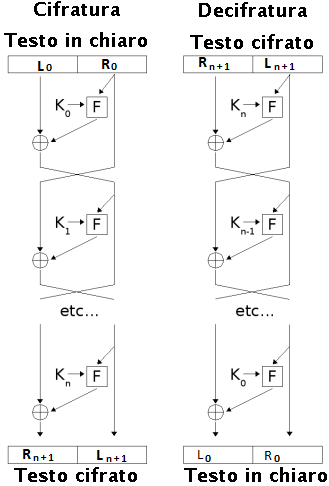
\includegraphics[scale = 0.6]{images/Feistel}
	\caption{Cifratura di Feistel.}
	\label{img:Feistel}
\end{figure}\\
In Figura \ref{img:Feistel} è riportato il processo di cifratura di Feistel. La struttura inventata da Feistel ha un vantaggio: cifratura e decifratura sono operazioni molto simili, spesso identiche, e basta invertire il funzionamento del gestore della chiave per ottenere l'operazione inversa; i circuiti di cifratura e decifratura, dunque, spesso sono gli stessi. Dalla chiave $K$ si generano una serie di sottochiavi $K_i$, $i=0,\dots,n$, attraverso una funzione generatrice. Si eseguono quindi una serie di fasi di cifratura che hanno come parametro $K_i$ ed il risultato della fase precedente. Vediamo brevemente nel dettaglio i passi di cifratura e decifratura.\\
Sia $F$ la funzione dei passaggi e siano $K_0, K_1, \dots, K_n$ le sottochiavi rispettivamente dei passaggi $0,\dots,n$. Le operazioni basilari sono le seguenti:
\begin{enumerate}
	\item Dividere i dati in ingresso in due parti uguali $(L_0, R_0)$.
	\item Per ogni round $i=1,2,\dots,n$, calcola
	\begin{align*}
		L_i &= R_{i-1} \\
		R_i &= L_{i-1} \oplus f(R_{i-1}, K_{i-1})
	\end{align*}
	dove $f$ è la funzione del round e $K_i$ è la chiave corrente. Si ottiene il testo cifrato $(L_{n+1}, R_{n+1})$.
\end{enumerate}
La decifratura si ottiene con:
\begin{align*}
	R_{i-1} &= L_i \\
	L_{i-1} &= R_i \oplus f(L_i, K_i)
\end{align*}
Un vantaggio di questo modello è che le funzioni $f$ usate sono \textit{non invertibili} e possono essere molto complesse. Il diagramma in Figura \ref{img:Feistel} mostra la cifratura e la decifratura del messaggio. Si noti l'inversione della chiave di sessione per la decifratura: è l'unica differenza rispetto alla cifratura del messaggio. Tutti gli algoritmi a blocchi moderni come AES usano questo schema di cifratura. 

\textbf{Oss.} Il DES non è basato sulla cifratura di Feistel, ma è una rete a sostituzione e permutazione a blocchi.

\section{Altri algoritmi}

\subsection{ID-based cryptography}
La crittografia basata sull'identità (IBC) è un tipo di crittografia a chiave pubblica in cui una stringa nota pubblicamente che rappresenta un individuo od un'organizzazione viene utilizzata come chiave pubblica. Tale stringa potrebbe includere un indirizzo e-mail, un nome di dominio od un indirizzo IP fisico.

Il problema di distribuire i certificati è un limite significativo della cifratura a chiave pubblica; impone un'infrastruttura e introduce costi di set-up di una sessione. La ID-based cryptography nasce per eliminare questo limite. Con IBC la chiave pubblica di un utente è derivata direttamente da un identificativo dell'utente, ad esempio $e=\text{hash}(\textsf{leonardo.maccari@unifi.it})$. Non vi è necessità di scambiarsi i certificati: il canale di trasmissione (e-mail, IP, etc.) definisce esso stesso l'associazione chiave-utente.\\
Tecnicamente esistono ancora molti limiti perché IBC prenda piede. Uno su tutti è che affinché il sistema funzioni è necessario che le chiavi vengano generate tutte da un ente fidato, al contrario di RSA in cui la chiave privata può non essere mai rivelata a nessuno se non al proprietario. Esistono comunque aziende che vendono soluzioni basate su IBC (e.g. Trend Micro).

\subsection{Quantum cryptography}
È una tecnica molto nuova, ma allo stato attuale non è molto utilizzata. Sostanzialmente si basa sull'utilizzo di informazioni modificabili associate ad una trasmissione di dati. Ad esempio, in una fibra ottica, l'arrivo di un fotone implica la ricezione di un'informazione. Ogni fotone possiede uno stato di polarizzazione che secondo il principio di indeterminazione di Heisenberg non può essere misurato senza interferirci. Negli stati dei fotoni viene codificata una chiave simmetrica che verrà utilizzata per cifrare il resto della comunicazione. Ad oggi si applica solo a comunicazioni su fibra.\\
Si noti infine che su fibra ottica non è possibile un man-in-the-middle: l'attaccante dovrebbe rompere fisicamente la fibra per farlo.

\subsection{Crittografia a chiave ellittica}
Dopo l'introduzione di RSA e Diffie-Hellman, sono state prese in considerazioni altre soluzioni matematiche per creare algoritmi che si servono di funzioni \textquotedblleft furbe". Nel 1985, gli algoritmi crittografici proposti si basavano su una branchia della matematica che studiava le \textit{curve ellittiche}. Sotto alcune condizioni particolari, un gruppo può essere definito da una curva ellittica, una curva piana definita da un'equazione del tipo $y^2 = x^3 + ax + b$. La \textit{crittografia ellittica} è una tipologia di crittografia a chiave pubblica basata sulle curve ellittiche definite su campi finiti. Ragionamenti analoghi a quelli fatti per RSA possono essere riportati al contesto delle curve ellittiche. Il problema del logaritmo discreto utilizzato nella crittografia (i.e. la funzione trappola, in questo caso la curva ellittica) a curva ellittica è molto più difficile del problema della fattorizzazione di numeri primi, a parità di dimensione del campo, e quindi a parità di sicurezza questa crittografia richiede chiavi pubbliche di dimensione inferiore, dunque più facilmente utilizzabili (operazioni di codifica e decodifica più semplici) rispetto a quelle utilizzate dal metodo RSA. La National Security Agency (NSA) americana ha inserito alcuni algoritmi a curve ellittiche nel \textit{suite} $B$, un insieme di algoritmi ufficialmente supportati. Vediamo più nel dettaglio come funziona la crittografia ellittica.
\begin{figure}[htbp]
	\centering
	\begin{tikzpicture}[domain=-1.769292354238631:2.5, samples at = {-1.32471795724475, -1.32, ..., 2.26}]
		\draw[->] (-2.2,0) -- (3.2,0) node[right] {$x$};
		\draw[->] (0,-2.2) -- (0,4.2) node[above] {$y$};
		\draw[-, color=blue] plot (\x,{sqrt(\x^3-\x+1)}) node[right] {$y^2=x^3-x+1$};
		\draw[-, color=blue] plot (\x,{-sqrt(\x^3-\x+1)}) node[right] {};
	\end{tikzpicture}
	\caption{Esempio di curva ellittica di equazione $y^2 = x^3 - x + 1$.}
	\label{img:elliptic_curve}
\end{figure}\\
Uno dei motivi fondamentali per cui le curve ellittiche hanno preso piede è che, rispetto alla fattorizzazione, la maggior parte delle persone (esperti compresi) non conosce molto bene la difficile matematica che sta dietro, ossia non è ben nota. Come già detto, una curva ellittica è l'insieme dei punti $(x, y) \in \mathbb{R}^2$ che soddisfano l'equazione $y^2 = x^3 + ax + b$; un esempio è riportato in Figura \ref{img:elliptic_curve}. Essa possiede alcune proprietà che la rendono una buona scelta nell'ambito della crittografia.\\
Una di queste è la simmetria orizzontale, ossia rispetto all'asse $x$. Qualunque punto sulla curva può essere riflesso attraverso l'asse $x$ ed il valore funzionale rimane invariato.\\
Una proprietà più interessante è che qualunque linea non verticale (eccetto alcuni casi particolari) interseca la curva in al più tre punti. Immaginiamo questa curva come un tavolo da biliardo. Prendiamo due punti qualsiasi sulla curva e tracciamo il segmento che li congiunge; la linea intersecherà la curva in più di un punto. Nel gioco del biliardo, invece, si prende una palla nel punto $A$ e si colpisce verso il punto $B$. Quando colpisce la curva, la palla rimbalza o verso l'alto (se è sotto l'asse $x$) o verso il basso (se è al di sopra dell'asse $x$) verso l'altro lato della curva. È abbastanza intuitivo capire che è molto difficile trovare il numero di volte in cui la palla rimbalza da un punto iniziale $A$ ad un punto finale $B$, conoscendo solo $A$ e $B$. In termini matematici e crittografici, si sta parlando quindi di una funzione interessante: è semplice da calcolare, ma è estremamente difficile tornare indietro.

In questo processo non abbiamo tenuto conto tuttavia di una cosa fondamentale: lavorando in un dominio discreto come quello di un calcolatore non è possibile rappresentare una funzione continua. A questo scopo vengono presi in considerazione solo valori interi in un intervallo fissato. Quando si calcola la formula per una curva ellittica si usa lo stesso trucco di \textquotedblleft ribaltare" i numeri quando raggiungiamo il massimo; se vincoliamo il massimo ad essere primo, la curva ellittica è chiamata \textquotedblleft curva prima" e possiede delle eccellenti proprietà crittografiche. Torniamo alla curva in Figura \ref{img:elliptic_curve}: essa è rappresentata per tutti i numeri reali.
\begin{figure}[htbp]
	\centering
	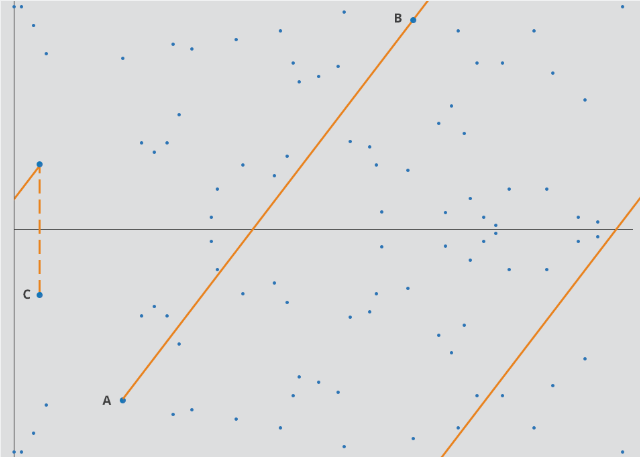
\includegraphics[scale = 0.5]{images/elliptic_curve_discrete}
	\caption{Esempio di discretizzazione della curva $y^2 = x^3 - x + 1$ con soli numeri interi rappresentati fino a 97.}
	\label{img:elliptic_curve_discrete}
\end{figure}\\
In Figura \ref{img:elliptic_curve_discrete} è rappresentata la stessa curva con i soli numeri interi rappresentati fino ad un massimo di 97. Anche se non sembrerebbe, essa rappresenta sempre una curva in senso tradizionale: è come se la curva originale fosse avvolta intorno ai bordi e solamente le parti della curva che \textquotedblleft colpiscono" i numeri a coordinate intere risultano colorate. È ancora possibile notare la simmetria orizzontale.

Con questa nuova rappresentazione della curva è possibile rappresentare i messaggi come punti su essa. Possiamo immaginare di prendere un messaggio ed assumerlo come coordinata $x$ per poi calcolare la $y$ ed ottenere un punto sulla curva; in realtà il processo è più complicato in pratica, ma l'idea di base è questa.

Ricapitolando, quindi, un sistema crittografico basato su curva ellittica può essere definito prendendo un numero primo come massimo, un'equazione di una curva ellittica ed un punto \textit{pubblico} sulla curva. Una \textit{chiave privata} è un numero $priv$ ed una chiave pubblica è ottenuta facendo \textquotedblleft rimbalzare" il punto pubblico su sé stesso $priv$ volte. Per il calcolo della chiave privata a partire dalla chiave pubblica in questo tipo di sistema crittografico deve essere utilizzata la funzione logaritmo discreto sulla curva ellittica: questa è la \textit{funzione trappola} che cercavamo. Tuttavia, proprio il fatto che la matematica che sta dietro a queste idee non è ben nota, si sospetta che la scelta \textquotedblleft errata" di alcuni parametri iniziali (ad esempio $a, b$ nell'equazione della curva) porti a dei risultati non molto robusti. Non è stato dimostrato, ma solo ipotizzato, che alcuni numeri portino a risultati veramente facili da decodificare.

La crittografia ellittica è estremamente facile da implementare ed attualmente è utilizzata in molti ambiti eccetto che per la codifica di dati sensibili, a causa proprio della mancanza di conoscenza della matematica alla base.

\newpage
\section{Organizzazione di una rete con certificati (esempio)}
La nostra rete, mostrata in Figura \ref{img:network_example1}, è composta da:
\begin{itemize}
\item Una rete di computer fissi per gli utenti
\item Un server per applicativi web necessari aigli utenti
\item Un server per la posta elettronica
\item Dei possibili utenti remoti (roadwarrior)
\end{itemize}

\begin{figure}[h]
	\centering
	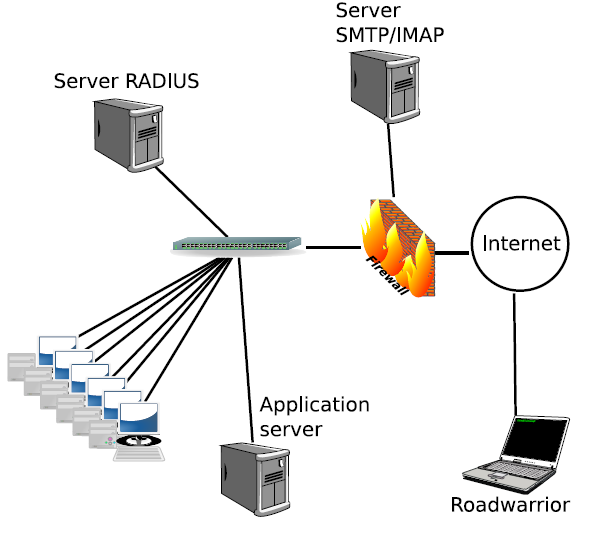
\includegraphics[scale = 0.4]{images/network_example1.png}
	\caption{Esempio di Rete}
	\label{img:network_example1}
\end{figure}

Nella nostra rete vogliamo assicurare che non sia possibile collegari alla rete interna se non utilizzando i client fissi della rete dal personale autorizzato. I servizi di webserver devono essere accessibili solo dai terminali della rete e la posta deve essere certificata in modo che gli utenti possano inviare e ricevere le email in modo semplice e sicuro. Inoltre tutto quello che può fare un utente interno alla rete lo deve anche poter fare il roadwarrior. Si può vedere come questi requisiti siano impegnativi da implementare e rispettare. \\

Per prima cosa abbiamo bisogno di una CA. Questa deve essere il più possibile isolata dalla rete e non accessibile dall'esterno o dagli utenti. La CA distribuisce certificati (e le rispettive CRL) agli utenti e ai server.  In particolare abbiamo bisogno dei seguenti certificati:
\begin{itemize}
\item Uno per il webserver (protocollo HTTPS)
\item Uno per il server imap e smtp per la posta elettronica
\item Uno per l'autenticazione degli utenti
\item Uno per la VPN in modo che i roadwarrior possano usare la rete interna
\item Uno per ogni macchina client, per ogni utente e per ogni roadwarrior
\end{itemize}

\newpage 

\begin{figure}[htbp]
	\centering
	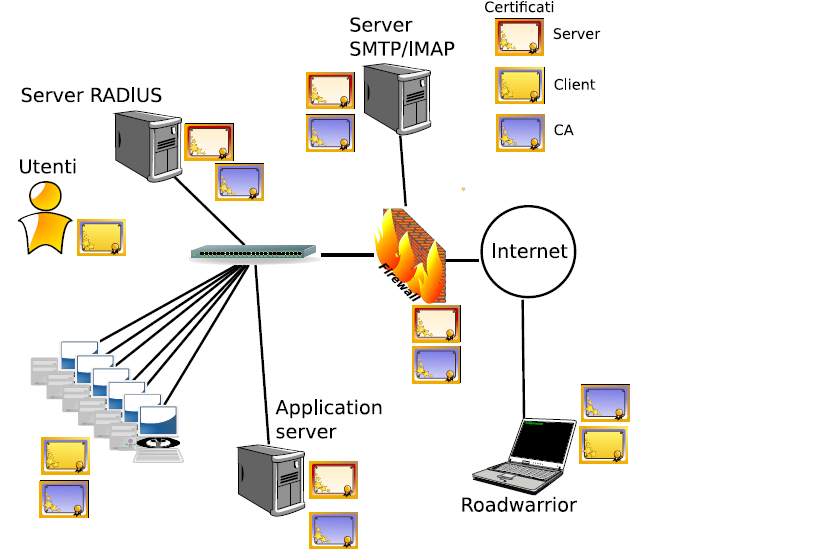
\includegraphics[scale = 0.4]{images/network_example2.png}
	\caption{Rete finale con i certificati}
	\label{img:network_example2}
\end{figure} 

Dove devo mettere i certificati segli utenti? Ogni macchina nella rete interna deve possedere un certificato non accessibile dall’utente. All’avvio la macchina dovrà produrre un’autenticazione con un server di autenticazione in modo da poter accedere allo switch a cui è collegata. C’è bisogno quindi di uno switch compliant con IEEE 802.1X e di un server RADIUS (vd. Capitolo 6). Ogni utente riceve un certificato (in una smartcard, o in un token di qualisasi tipo), i terminali utenti devono avere un lettore hardware. Quando l’utente arriva alla postazione si autentica con il token allo stesso server RADIUS e ottiene il login. Lo stesso certificato verrà utilizzato dai client di posta elettronica e dal webserver. Volendo, oltre al certificato, il login può essere legato anche ad una password, utilizzabile direttamente dal token crittografico per sbloccarsi. Infine tutti gli utenti, i server e le VPN deveno avere il certificato della CA insieme alla CRL. La rete finale è illustrata in Figura \ref{img:network_example2}.


